\documentclass[a4paper,10pt,oneside]{article}
\usepackage{graphicx}
\usepackage{color}
\usepackage{url}
\usepackage{subfigure}
\usepackage[utf8]{inputenc}
\usepackage[T1]{fontenc}
\usepackage{tgpagella}
%\usepackage[scale=0.9]{tgcursor}
%\usepackage[scale=0.9]{tgheros}
\usepackage{xstring}

\newcommand{\myscale}{0.74}
\newcommand{\vect}[1]{\boldsymbol{#1}}
\newcommand{\code}[1]{\texttt{\StrSubstitute{#1}{.}{.\.}}}
\def\.{\discretionary{}{}{}}
\newcommand{\jmodule}[1]{\texttt{\textit{#1}}}

\setlength{\hoffset}{-1in} %left margin will be 0, as hoffset is by default 1inch
\setlength{\voffset}{-1in} %analogous voffset
\setlength{\oddsidemargin}{1.5cm}
\setlength{\evensidemargin}{1.5cm}
\setlength{\topmargin}{1.5cm}
\setlength{\textheight}{24cm}
\setlength{\textwidth}{18cm}

\def\mftitle{jInfer AutoEditor Module Description}
\def\mfauthor{Michal Klempa, Mário Mikula, Robert Smetana, Michal Švirec, Matej Vitásek}
\def\mfadvisor{RNDr. Irena Mlýnková, Ph.D., Martin Nečaský, Ph.D.}
\def\mfplacedate{Praha, 2011}
\title{\bf\mftitle}
\author{\mfauthor \\ Advisors: \mfadvisor}
\date{\mfplacedate}

\ifx\pdfoutput\undefined\relax\else\pdfinfo{ /Title (\mftitle) /Author (\mfauthor) /Creator (PDFLaTeX) } \fi

\begin{document}
\maketitle
\noindent Target audience: developers willing to extend jInfer, specifically alter displaying of automata .

\noindent \begin{tabular}{|l|l|} \hline
Responsible developer: & Mário Mikula \\ \hline
Required tokens:       & org.openide.windows.WindowManager \\ \hline
Provided tokens:       & none \\ \hline
Module dependencies:   & Base \\ 
					   & JUNG \\ \hline
Public packages:       & cz.cuni.mff.ksi.jinfer.autoeditor \\ 
					   & cz.cuni.mff.ksi.jinfer.autoeditor.automatonvisualizer \\
   					   & cz.cuni.mff.ksi.jinfer.autoeditor.automatonvisualizer.layouts \\
   					   & cz.cuni.mff.ksi.jinfer.autoeditor.gui.component \\ \hline
\end{tabular}

\section{Introduction}

This is an implementation of a \jmodule{AutoEditor}. Using JUNG library, it provides an API to display and user interactively modify automata, thus the process of inference can be easily made user interactive.

TODO spomenut vsade packages

TODO UML diagramy su zjednodusene z dovodu prehladnosti

\section{Structure}

Structure of \jmodule{AutoEditor} can be divided into following four main parts.

\begin{itemize}
	\item API - API to display automaton in GUI.
	\item Base classes - Classes providing basic functionality that can be extended and combined to achieve desired visualization of an automaton.
	\item Derived classes - Classes derived from the base classes that are used in existing modules and simultaneously serve as examples.
	\item Layout creation - System of creating \code{Layout}s.
\end{itemize}

First, \code{Layout}s and use of base classes to create a visualization of automaton will be described.

\subsection{Layout}

\code{Layout} is a JUNG interface responsible primarily of representation of automaton and positions of its states. JUNG library provides several implementation of \code{Layout} interface. However, none of them is convenient for automatic automaton displaying, \jmodule{AutoEditor} provides two additional implementations. \code{Layout} by \emph{Julie Vyhnanovska}, used in her master thesis and \code{Layout} which is using external \emph{Graphviz} software. TODO odkazy v predchadzajucej vete.\\

Class providing creation of \code{Layout} instances is named \code{LayoutHelperFactory}.

\subsubsection{Vyhnanovska Layout} \label{subsubsection:vyhnanovskaLayout}

As mentioned above, this Layout was implemented by \emph{Julie Vyhnanovska} as a part of her master thesis. TODO link? It positions automaton states to a square grid. This \code{Layout} gives good results for relatively small automata (about 10 states of less) but for larger ones, the results are quite disarranged and confused.\\

Source codes resides in package \code{cz.cuni.mff.ksi.jinfer.autoeditor.automatonvisualizer.layouts.vyhnanovska}.

\subsubsection{Graphviz Layout} \label{subsubsection:graphvizLayout}

\code{Graphviz Layout} uses \emph{Graphviz}, third-party graph visualization software, to create positions of automaton states. TODO link? To use this \code{Layout}, \emph{Graphviz} has to be installed and path to \emph{dot} binary has to be set in options. This \code{Layout} gives nice results even on large automata.\\

TODO ako presne ziskava pozicie z graphvizu

Source codes resides in package \code{cz.cuni.mff.ksi.jinfer.autoeditor.automatonvisualizer.layouts.graphviz}.

\subsubsection{LayoutHelperFactory} \label{subsubsection:LayoutHelperFactory}

In project properties, it is possible to select a \code{Layout} to be used to display automata. \code{LayoutHelperFactory} is class, providing just one static method, responsible for creating instances of \code{Layout}s according to a selection in project properties.\\

This method has following signature.

\begin{verbatim}
public static <T> Layout<State<T>, Step<T>> createUserLayout(final Automaton<T> automaton, final Transformer<Step<T>, String> edgeLabelTransformer) throws InterruptedException;
\end{verbatim}

The first argument is a automaton to create a layout from. The second is transformer to transform an instance of automaton edge to its string representation, required by the \code{Graphviz Layout}.

Source codes resides in package \code{cz.cuni.mff.ksi.jinfer.autoeditor.automatonvisualizer.layouts}.

\subsubsection{How to create a new Layout}

\code{Layout}s can be implemented using the modular system. To create a new implementation of \code{Layout} interface, it is needed to create a new class implementing \code{LayoutFactory} interface (package \code{package cz.cuni.mff.ksi.jinfer.autoeditor.automatonvisualizer.layouts}) and annotate it by the following code.

\begin{verbatim}
@ServiceProvider(service = LayoutFactory.class)
\end{verbatim}

Created implementation will be shown in project properties in the \code{Layout} selection.\\

System of modules is described in detail in TODO ref.

\subsection{Base classes}

This section describes classes implementing basic common functionality that are supposed to be extended to create a new suitable visualization of automata for a particular method of inference. The new visualization may involve a brand new GUI panel with buttons with various functions, user interaction like selecting states or edges and others.\\

Main two classes representing visualization of automaton are \code{Visualizer} and \code{AbstractComponent}. \code{Visualizer} is a graphical representation of automaton and \code{AbstractComponent} is a panel (extends \code{JPanel}) containing the \code{Visualizer} which will be displayed in GUI.
TODO obrazok ako AC dedi od JPanelu a obsahuje Visualizer.

\subsubsection{Visualizer}

\code {Visualizer} class extends JUNG \code{VisualizationViewer} class thus it provides all its methods and adds support for saving contained automaton to an image file. Responsible methods are \code{saveImage()} and \code{getSupportedImageFormatNames()}. However, to save an image of automaton it is not necessary to call this methods directly. \jmodule{AutoEditor} GUI contains button to save an image of displayed automaton. For information on how to to this, see TODO ref.\\

Constructor has one argument, instance of \code{Layout} interface created from an automaton, typically by \code{LayoutHelperFactory} (see \ref{subsubsection:LayoutHelperFactory}).

\subsubsection{PluggableVisualizer}

\code{PluggableVisualizer} class is extension of \code{Visualizer} class, which primarily provides an easy way to plug \emph{graph mouse plugins}.\\

\emph{Graph mouse plugin}s are classes implementing JUNG \code{GraphMousePlugin} interface and their purpose is to enhance \code{Visualizer} with mouse support.\\

By default, instance of \code{PluggableVisualizer} is constructed with two plugins enabled. They are \code{ScalingGraphMousePlugin}, providing zooming, and \code{TranslatingGraphMousePlugin}, providing translating the displayed automaton in the x and y direction. In the most cases, these plugins are useful but if they are not wanted they can be removed using methods \code{getGraphMousePlugins()} and \code{removeGraphMousePlugin()}.\\

TODO obrazok ako PluggableVisualizer dedi od Visualizeru

Public (not inherited) methods of \code{PluggableVisualizer} are the following. Their purpose is clear from their names, for details see their JavaDoc.

\begin{itemize}
	\item \code{addGraphMousePlugin()}
	\item \code{removeGraphMousePlugin()}
	\item \code{getGraphMousePlugins()}
	\item \code{replaceVertexLabelTransformer()}
	\item \code{replaceEdgeLabelTransformer()}
\end{itemize}

\subsubsection{AbstractComponent}

\code{AbstractComponent} class is a representation of GUI panel containing an instance of \code{Visualizer} class for some automaton. It is inherited from \code{JPanel} class thus provides JPanel's method and behaviour. In addition, it provides the following methods.

\begin{itemize}
	\item \code{setVisualizer()} - Setter of \code{Visualizer}.
	\item \code{getVisualizer()} - Getter of \code{Visualizer}.
	\item \code{waitForGuiDone()} - Suspends its thread until method \code{guiDone} is called on this instance. Do not call this method directly, it is called by \jmodule{AutoEditor}. For more information, see \ref{subsubsection:AbstractComponent user-interactivity support}.
	\item \code{guiDone()} - Wakes up this instance from a suspended state. For detailed description, see \ref{subsubsection:AbstractComponent user-interactivity support}.
	\item \code{guiInterrupt()} - Called when \jmodule{AutoEditor}'s tab is closed to propagate information about terminating of inference to a caller of \jmodule{AutoEditor}. There is no need to called this method directly.
	\item \code{guiInterrupted()} - Checks if \jmodule{AutoEditor} GUI was terminated by interrupt or regularly. Also, there is no need to call this method directly, it is called by \jmodule{AutoEditor}. For details, see TODO ref GUI.
\end{itemize}

Besides those methods, \code{AbstractComponent} has one abstract method, named \code{getAutomatonDrawPanel()}.\\

Purpose of this class is to be extended to create own GUI panel, which displays some automaton using a supplied instance of \code{Visualizer}. Method \code{getAutomatonDrawPanel()} is meant to be overridden to returns an instance of \code{JPanel}, in which the \code{Visualizer} is to be drawn.\\

Programmer implementing an extension of \code{AbstractComponent} is not forced to place the \code{Visualizer} on its own. It is just needed to create \code{JPanel} and define \code{getAutomatonDrawPanel()} method to return this \code{JPanel}. \jmodule{AutoEditor} will take care of placing and displaying the \code{Visualizer} in the \code{JPanel}.\\

\code{Visualizer} is not set in constructor, because it is often desired to subsequently display several different automata (\code{Visualizer}s) in the same panel. In this case it is not needed to create new instance of \code{AbstractComponent} for each \code{Visualizer}, but subsequently call \code{setVisualizer()} method using one instance of \code{AbstractComponent}.

\begin{figure}
\centering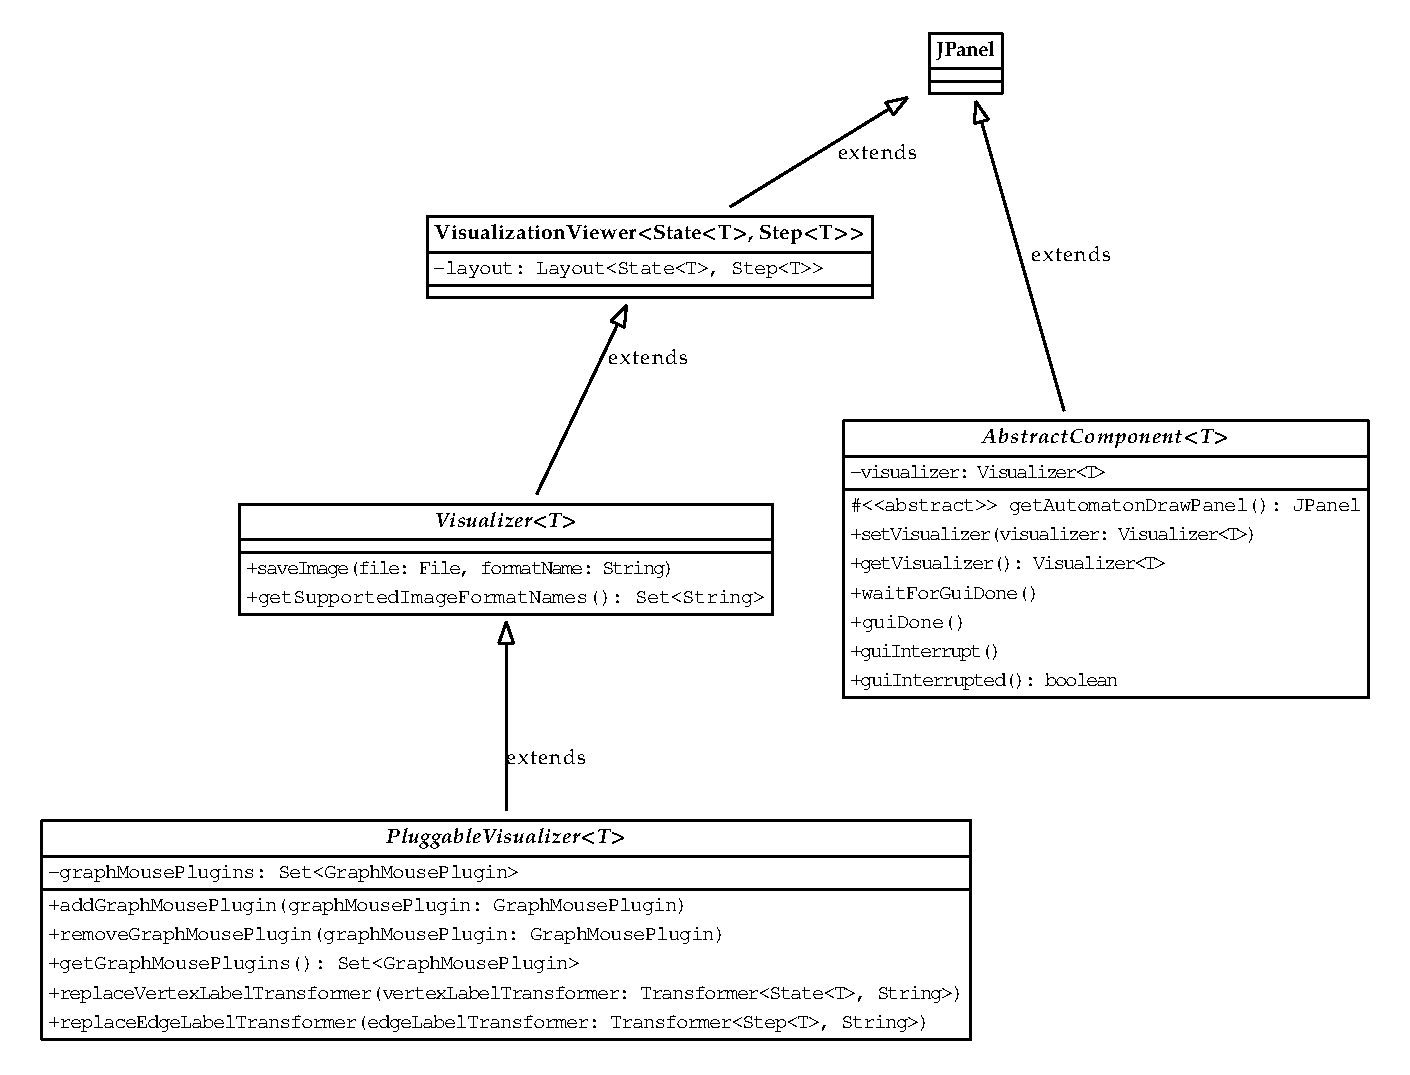
\includegraphics[scale=\myscale]{uml_basic_full}
\caption{Class diagram for the base classes.} \label{uml_basic_full}
\end{figure}

\subsubsection{AbstractComponent user interactivity support} \label{subsubsection:AbstractComponent user-interactivity support}

If some kind of user interactivity is desired, \code{AbstractComponent} is a right place to implement it.\\

To display the component in GUI and wait for some user action, method \code{waitForGuiDone()} is used. After displaying the component, calling of this method suspend running thread thus code execution of a caller module is stopped at the place of this call. However, GUI is ran in another thread, user is able to interact with the panel (component).\\*
Do not call method \code{waitForGuiDone()} directly. It is called by \jmodule{AutoEditor} when displaying the component by \jmodule{AutoEditor} \emph{API} method named \code{drawComponentAndWaitForGUI()}. For more information on \jmodule{AutoEditor} \emph{API}, see TODO ref.\\

Method important for a programmer extending \code{AbstractComponent} is named \code{guiDone()}. This method wakes up the thread suspended in \code{waitForGuiDone()} method and the programmer is responsible for calling it. Typically, it is called upon some user action like button click, vertex pick or other GUI event.\\*
After calling of \code{guiDone()} method, code execution of the caller module is resumed and holding instance of the \code{AbstractComponent} it is able to retrieve results of user interaction, saved in its state.\\

For examples of user-interactive component, see TODO ref. 

\subsection{API}

\jmodule{AutoEditor} \emph{API} is pretty simple. Package \code{cz.cuni.mff.ksi.jinfer.autoeditor} contains class \code{AutoEditor} with three public static methods.

\begin{itemize}
	\item \code{drawComponentAsync()} - Displays given \code{AbstractComponent} asynchronously in a GUI thread and immediately returns. Use this method to just display automaton, without any user interaction and without waiting for any external event. This method does not support these.
	\item \code{drawComponentAndWaitForGUI()} - Displays given \code{AbstractComponent} in a GUI thread and a caller thread is suspended until  \code{guiDone()} method of \code{AbstractComponent()} is called. This method can wait for GUI events thus is convenient for user interaction. How to achieve it is described in detail in \ref{subsubsection:AbstractComponent user-interactivity support}.
	\item \code{closeTab()} - Closes \jmodule{AutoEditor}'s GUI tab and interrupts inference, if running.
\end{itemize}

For examples of API usage, see TODO ref.

\subsection{Derived classes}

\begin{figure}
\centering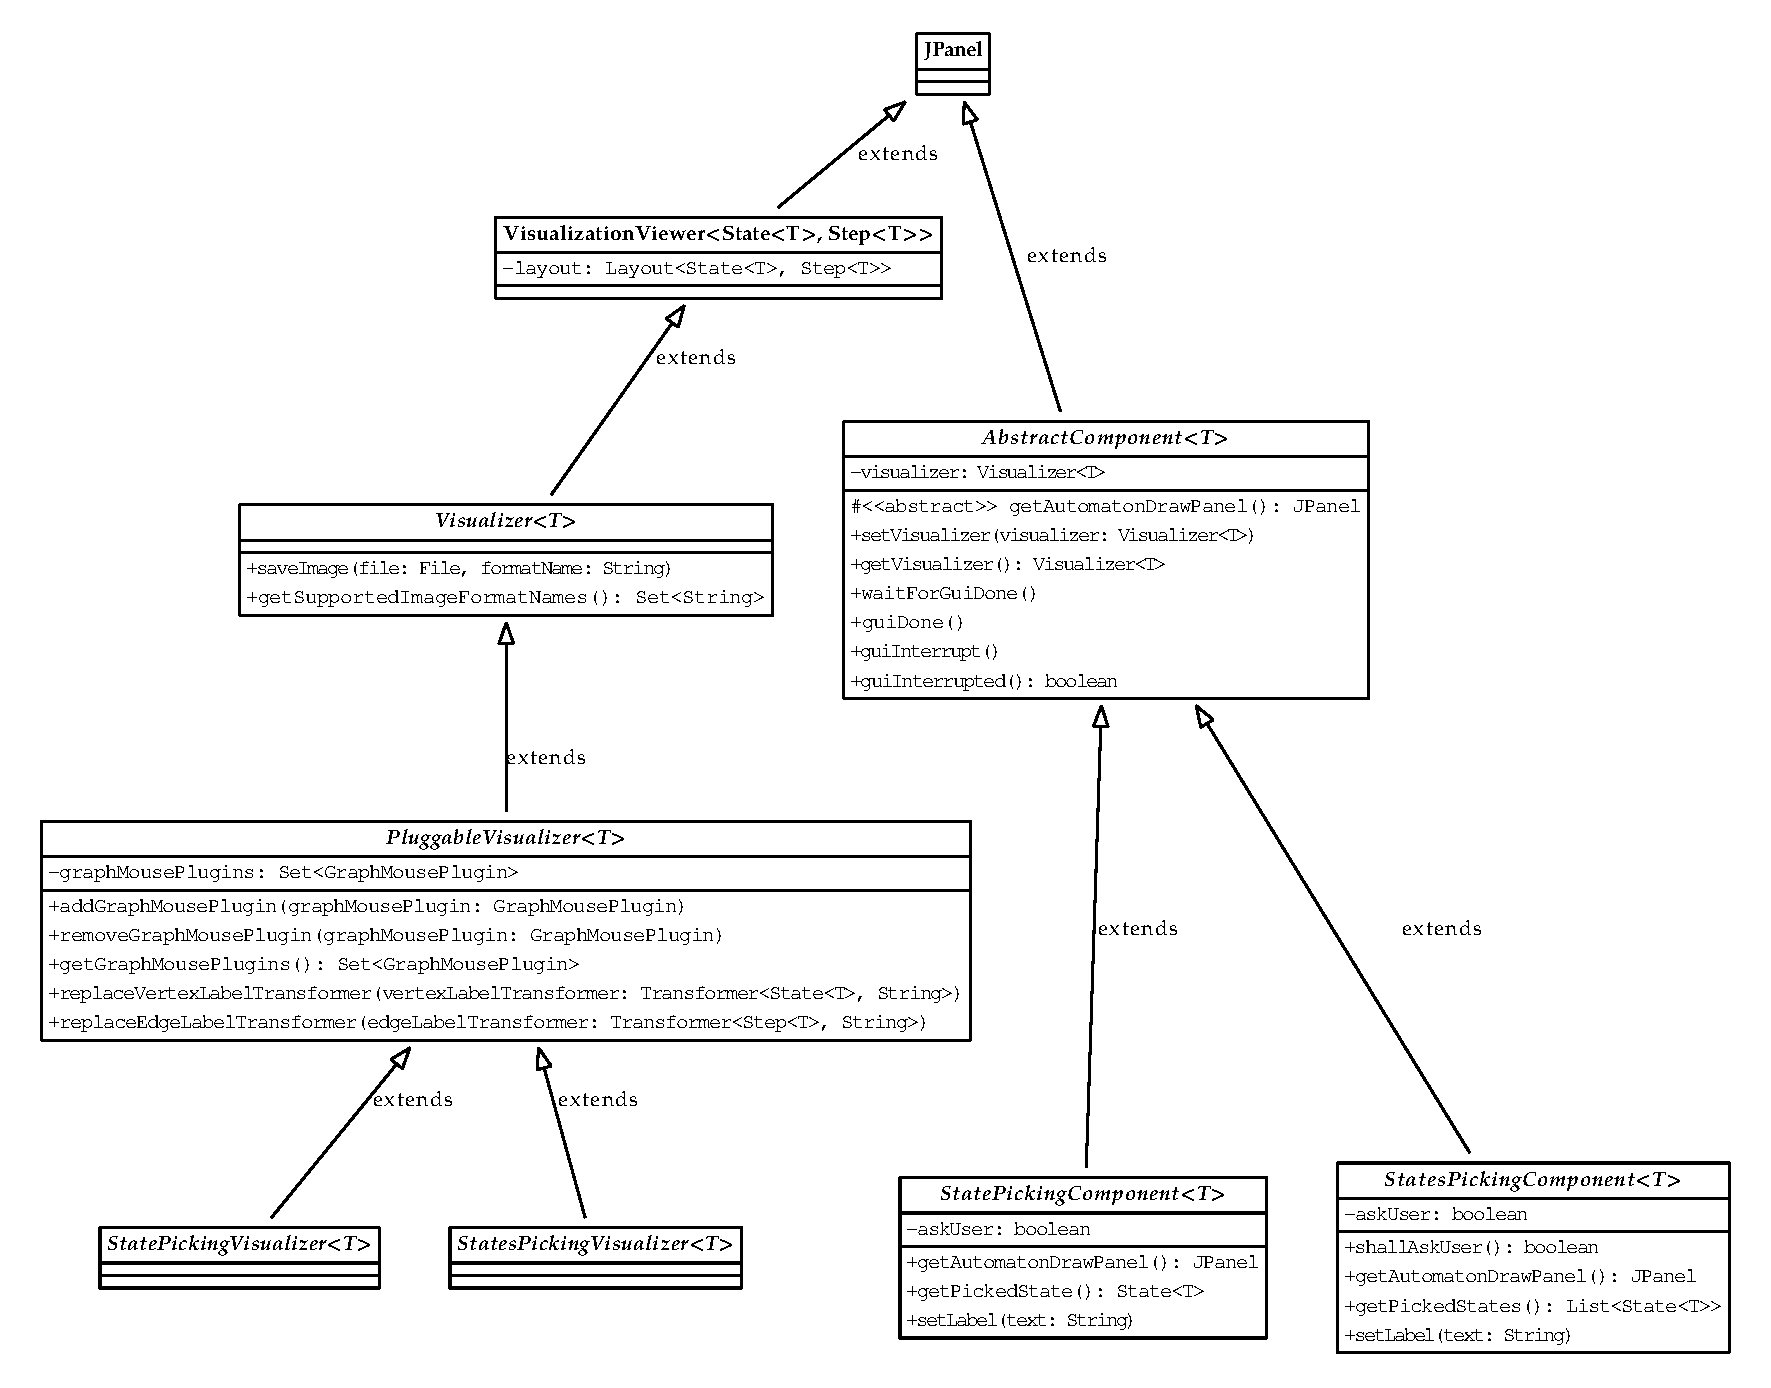
\includegraphics[scale=\myscale]{uml_derived_classes}
\caption{Class diagram for the derived classes.} \label{uml_derived_classes}
\end{figure}

Popis tried pouzitych v inych moduloch, ktore sluzia zaroven ako priklad.

StatePickingVisualizer
StatesPickingVisualizer

\subsection{GUI}

TODO

tlacitka

\subsection{Preferences}

TODO

All settings provided by \jmodule{BasicXSDExporter} are project-wide, the preferences panel is in \code{cz.cuni.mff.ksi.jinfer.basicxsd.properties} package. As mentioned above, it is possible to set the following. 

\begin{itemize}
	\item Turn off generation of global element types. Turning off this feature is not recommended as it may cause certain problems with validity of resulting XSD. See \ref{section:problems}.
	\item Minimal number of occurrences of element to define its type globally. (Only if generation of global elements is active.)
	\item Number of spaces in output per one level of indentation.
	\item Global type name prefix. It is a string which will be inserted before a name of a type, which is derived from element's name. Can be also an empty string. (Only if generation of global elements is active.)
	\item Global type name suffix. It is a string which will be appended after a name of a type, which is derived from element's name. Can be also an empty string. (Only if generation of global elements is active.)
\end{itemize}


\nocite{*}
\newpage
\bibliographystyle{alpha}
\bibliography{literature}

\end{document}
